% SPDX-FileCopyrightText: 2026 Hasan Melih Akbulut
% SPDX-License-Identifier: CC-BY-4.0

\chapter{The neuromorphic accelerator}
\label{ch:npu}

This block exists in two sizes at once. There is a full-scale
specification --- 512 neurons, 512 axons, a quarter of a million
synapses in an error-corrected SRAM --- written as \dcite{10}{}, dated
24 August 2026, with a bit-exact Python golden model as its normative
executable form. And there is a slice of it, elaborated at eight
neurons and eight axons with its synapses in flip-flops, carried
through synthesis, placement, routing and geometric sign-off and
submitted to a Tiny Tapeout shuttle, where \dcite{34}{} pins every byte
of it by hash. Everything measured here was measured on that slice or
on the system-on-chip that instantiates it.

\section{What it computes: leaky integrate-and-fire, in integers}

The neuron model is classical digital leaky integrate-and-fire
\cite{frenkel2019}. Each
neuron carries a 24-bit state word: a signed 16-bit membrane potential
\code{V}, an unsigned 4-bit refractory countdown \code{R}, and four
reserved bits \dcite{10}{section 3} holds open as a per-neuron parity
hook. Threshold, reset potential, leak shift, synaptic shift and
refractory period are core-global configuration loaded once per pass,
not per-neuron state. \dcite{10}{section 4} states the update as ten
numbered equations (\cref{tab:npu-eqs}), and the discipline that
matters is that they are exact integer arithmetic with explicit
saturation --- no floating point anywhere in the evaluation path, by
construction and by test.

\begin{table}[tbp]
\centering
\caption{The normative update equations of \dcite{10}{section 4}, as
implemented in \code{hw/rtl/lif\_core.v} and in
\code{sw/golden/lif\_core.py}. The test
\code{sw/tests/test\_traceability.py} parses the specification for tags
and fails if one is uncovered, and, per a corrective note dated
2026-09-11, if the covering test asserts nothing.}
\label{tab:npu-eqs}
\small
\begin{tabularx}{\linewidth}{@{}lX@{}}
\toprule
\textbf{Tag} & \textbf{Contract} \\
\midrule
E1 & $w = \mathrm{sext4}(W[a][j])$, a 4-bit signed weight, $w \in [-8,+7]$ \\
E2 & $c = w \cdot 2^{S_{\mathrm{SYN}}}$, exact, $S_{\mathrm{SYN}} \in [0,7]$, so $c \in [-1024,+896]$ \\
E3 & $V' = \mathrm{sat16}(V + c)$, summed at full 18-bit signed width, then clamped \\
E4 & spike $\iff V' \geq \Theta$, signed, checked \emph{after} the update \\
E5 & on spike: $V \leftarrow V_{\mathrm{RESET}}$, $R \leftarrow T_{\mathrm{REFR}}$, emit id $\mathrm{TILE\_OFF}+j$ \\
E6 & leak toward zero by $\max(|V| \gg S_{\mathrm{LEAK}},\,1)$; the sign never flips \\
E7 & $R>0$ gates E1--E5 for that (event, neuron); a tick decrements $R$ \\
E8 & determinism: arrival order, ascending scan, spikes emitted in scan order \\
E9 & multi-pass neuron-tiling equivalence \\
E10 & an uncorrectable weight word substitutes $c=0$; processing continues \\
\bottomrule
\end{tabularx}
\end{table}

Three of the ten carry a decision rather than a definition.

\textbf{E3 saturates and must never wrap}, because a two's-complement
wraparound of a positive overflow would silently \emph{lose} a spike
rather than produce a wrong one, and a lost spike is invisible.

\textbf{E4 is checked after the update}, on every non-gated event,
including events whose contribution is zero. \dcite{10}{section 4.1}
calls checking before the update, or one event late, a specification
violation, for a stated reason: this exact off-by-one was a verified
bug class in the developer's prior integrate-and-fire silicon work.

\textbf{E6's leak has a minimum step of one}, so every non-zero
potential reaches zero within $|V|$ ticks rather than being stranded
once the shift rounds down. That bound licenses the project's position
on unprotected neuron state, which \dcite{10}{section 11.3} states as a
bet rather than a result: no error-correcting code on the membrane
potential in v0.1, because an upset in \code{V} costs at worst one
spurious or missed spike and then decays back toward rest --- on the
order of 100 ticks at the reset leak shift of 3 from full scale --- and
an upset in \code{R} costs at most $T_{\mathrm{REFR}} \leq 15$ ticks of
wrong gating. The four reserved bits are the hook if a campaign shows
the bet is wrong. The pilot did not wait for that: \code{lif\_core.v}
holds the 20-bit $\{R,V\}$ word under one SECDED $(26,20)$ codeword, six
check bits per neuron, so the elaborated slice corrects what the
specification leaves bare (\dcite{16}{section 2.1}).

E8 is what makes the rest possible: no arbitration, no clock-dependent
reordering, no dropped event on the processing path, so the core is a
deterministic function of state, configuration, weights and event
order. That is what lets a golden model be bit-exact against hardware
and a fault-injection verdict be attributable to the bit that was
flipped.

\section{Spikes on a wire: the address-event representation}

Events are 16-bit words and \dcite{10}{section 7.1} freezes the layout:
two bits of \code{TYPE}, four reserved zero bits, and a 10-bit
\code{ID} that is an axon identifier inbound and a neuron identifier
outbound. \code{TYPE} 00 is a \code{SPIKE}, 01 a \code{TICK} --- a
timestep boundary, which runs the leak and the refractory countdown and
emits nothing --- 10 a \code{SYNC}, and 11 is reserved, dropped and
counted. The core consumes time and does not create it: tick generation
is external in v0.1.

\code{SYNC} is the primitive the sequencing rests on: when one is
consumed, every prior event has been fully processed and the barrier is
echoed downstream, so a host injects one after a frame and reads until
it returns.

The queues are \code{hw/rtl/aer\_fifo.v}, 64 entries each in the
specification, and their contract is more interesting than their depth.
A write while full is dropped rather than allowed to corrupt stored
events or pointers, and counted in a sticky saturating counter
(\code{CNT\_EVQ\_OVF}); a link-side producer instead gets lossless
backpressure by gating its write with \code{!full}. Both pointers are
triple-redundant and voted. Every stored entry carries an even-parity
bit, \emph{detected and not corrected} --- a read whose word fails the
check discards the entry and holds \code{rd\_valid} low --- and that
signal is itself dual-rail and likewise detected, so a rail
disagreement reads low and the answer is missed rather than fabricated.
A full output queue stalls the update pipeline rather than dropping
spikes, and deadlock freedom across a mesh is assigned to a future
router.

\section{The crossbar and the weight memory}

Logically the synapses are a crossbar: $W[a][j]$ for axon $a$ and
neuron $j$, 4-bit signed, at bit address
$(a \cdot \mathrm{N\_NEURONS} + j)\cdot 4$ --- axon-major, so one
event's weight column is a contiguous burst. Physically, at full scale,
they are an SRAM with a single update pipeline time-multiplexed across
all neurons \cite{openspike2023}: \dcite{02}{section 3}'s Candidate~B, chosen because
flip-flop weights do not scale.

The physical word is 64 data bits, exactly 16 weights, plus 8 check
bits of a single-error-correcting double-error-detecting code
\cite{hsiao1970}: a 72-bit macro word at 12.5\,\% overhead. At the 512-by-512 default that is
16,384 words --- 128\,KB of data and 16\,KB of check bits, the dominant
area of the block (\dcite{10}{section 5}) --- and one synaptic event
reads 32 of them, the pipeline applying E1--E5 to 16 neurons per
word.

\textbf{That codeword is not the one the architecture study assumed,
and the correction is on the record rather than edited into it.}
\dcite{02}{section 2} carries a note dated 2026-09-09 saying its own
sizing used 32 data bits plus 7 check bits, and measuring the cost:
every figure derived from that document's 156\,KB is high by 8.33\,\%
of the 144\,KB basis. Nothing was renumbered, by the rule that a
superseded figure stays visible with a dated note saying what replaced
it (\dcite{64}{section 2}). What the note could not fix is that
\dcite{10}{section 5} calls its 144\,KB ``in line with the
\code{docs/02} estimate'' --- a claim of agreement across exactly that
8.33\,\%, in a document the note does not own. Both stand, and a reader
should treat them as disagreeing by that amount.

Single-bit errors are corrected inline and counted in \code{CNT\_SEC}.
A double-bit error takes E10: zero is substituted for every weight in
the affected word, \code{CNT\_DED} increments, \code{FAULT\_ADDR}
latches the word index, and processing continues. The core is
deliberately fail-operational --- a dead weight word degrades the
network rather than stopping the node --- and a background scrubber
walks the array while the input queue is empty, so single-bit errors do
not accumulate into double-bit ones \cite{saleh1990}.

\textbf{What the pilot stores is flip-flops, and that is a fallback
that was taken rather than a simplification.}
\code{hw/rtl/lif\_core.v}'s header states it: the synapse array is a
flip-flop file with a one-weight-per-cycle load port and no SRAM macro
--- \dcite{02}{section 3}'s Candidate~A storage class, reached by that
document's fallback trigger F1. The trigger fired for a measured
reason: \dcite{12}{sections 7.5 and 8} hardened one \code{RM\_IHPSG13}
macro \cite{ihppdk} and returned a \textsc{no-go} for this shuttle, because the macro
places, routes and closes timing and then fails Magic design-rule
checking, KLayout design-rule checking and Netgen
layout-versus-schematic on causes entirely inside the vendor views ---
1,106,478, 2,316 and 359 errors, as \dcite{61}{section 14} quotes them.
Dropping to flip-flops did not drop the code with it, so E10 is
implemented in the pilot at exactly the 16-weight granularity the
golden model's word index defines. The cost of time-multiplexing is in
the same header: one event or tick takes $\mathrm{N\_NEURONS}+1$ cycles
at full output bandwidth, independent of sparsity --- precisely the
trade that buys the memory scaling.

\section{Networks larger than the fabric}

The physical core holds one weight slice. Larger models live in flash
as a sequence of pass images: load the slice, load the configuration
and tile offset, replay the input event stream, collect output events
until the barrier returns. Sequencing is owned by the management core
through the register map in v0.1 (\dcite{10}{section 9}).

Output-neuron tiling is E9: partition a layer's output neurons into
ordered contiguous tiles, run one pass per tile with the matching
weight columns and the tile base in \code{PASS\_TILE\_OFF}, replaying
the identical input stream each time; concatenating the tiles'
emissions in tile order, per input event, gives a stream bit-identical
to a core wide enough for the whole layer. It holds because neuron
trajectories are mutually independent in v0.1 --- no lateral coupling.
The axon dimension is \emph{not} splittable, and the specification says
why rather than merely forbidding it: axon-split passes would
interleave saturation and threshold crossings in a different order and
break bit-exactness. Tiling does not lift the identifier bound either,
since the \code{ID} field and \code{PASS\_TILE\_OFF} are both ten bits,
so every tile must satisfy
$\mathrm{TILE\_OFF} + \text{tile width} \leq 1024$ --- a bound the
golden model enforces at construction, refusing wider layers rather
than approximating them.

\section{Attaching it to the system-on-chip}

Until \dcite{51}{} the repository held a RISC-V system-on-chip and a
separate accelerator that had never been in the same simulation. The
connection is built the hard way: \code{hw/rtl/pilot\_top.v}, the
frozen die's own top level, pinned by blob hash and unmodified, is
\emph{instantiated} inside \code{hw/soc/rtl/\allowbreak{}soc\_npu.v}
and reached over the same four serial pins the die will have. No copy
exists under \code{hw/soc/}, and a guard suite fails if any of the ten files
\dcite{34}{section 2.1} pins is edited against the index.

\subsection{Two faces, because there are two problems}

The node register window sits on the system bus: one 4\,KiB window per
mesh node, at the node index times \code{0x1000} --- the per-node base
address \dcite{10}{section 8} freezes --- reached with ordinary loads
and stores. The event port sits on the peripheral bus in a 4\,KiB slot
called \code{NPUCFG}: two 16-bit event queues with a hardware engine
between them and the die, plus the block's interrupt.

Nothing in the memory map moved to accommodate this, and everything
outside a live node's register block faults rather than aliasing: an
address above the sixteen windows, an uninstantiated node index, an
offset above \code{0x1FC} where the die's seven-bit register address
runs out, and a sub-word write --- because the serial frame carries no
byte enable, so a slave that accepted a byte store would write three
bytes of a register the master never named. Check 25 of the bring-up
program requires a fault for every one of them --- a load-access fault
at each of its five bad addresses, a store-access fault for the byte
store.

\subsection{Why the transport is serial}

The die's host port is serial because it was designed against a Tiny
Tapeout pin budget; inside a system-on-chip there is none, so a
parallel register port on a copy of the pilot was a real option.
\dcite{51}{section 3} argues the choice and rejects the obvious reason
--- ``the die will only have a serial port'' --- because a bench
harness for the die needs a serial host either way. What decides it is
that the serial transport leaves exactly \emph{one} implementation of
the die's host protocol, the one in the system-on-chip's own
regression, so the three host obligations the die numbers H1, H2 and H3
are implemented once and proved once. What was built is a level above a
memory-mapped serial master --- the address is the interface, the
transport is underneath it --- so a future node with the native 32-bit
configuration bus \dcite{10}{section 1} specifies is a change of
transport under an unchanged driver.

The cost is stated rather than waved at. A node-window register access
costs \textbf{176 clock cycles} from request to response, of which 171
is the serial frame; the protocol's arithmetic floor --- 40
serial-clock cycles plus one period of select setup and one of
inter-frame gap, at two clock cycles per half period --- is 168, and
the cocotb test asserts the measurement lies between the floor and the
floor plus 24, so the number is an observation and not a design intent
(\dcite{51}{section 8.1}). At full scale the same transport would need
32,768 register writes for one weight image, which is why
\dcite{10}{section 9} puts bulk loading on a flash path.

\subsection{The parallel event pins are not symmetric}

The die's event pins are used inbound and cannot be used outbound, and
both facts come from the pin contract. Inbound, the pin word's type
field comes from a single tick pin, so it is 00 or 01 and never 10:
\textbf{the barrier cannot be injected over the pins at all}, and goes
over the serial input-queue register instead, once per frame rather
than once per event. Outbound, the four-bit identifier pins carry no
type, so a barrier echo and a spike from neuron 0 are the same four
bits --- conflating exactly the event the sequencer depends on. So the
output-valid pin is a \emph{notification}, the word is read from the
die's output-queue register, and the acknowledge pin is tied low
because the serial read is itself the pop. The result is an asymmetry
of about 44 times --- four clock cycles inbound, a frame outbound ---
which \dcite{51}{section 4} attributes to the tile's pin budget rather
than to a design choice.

\subsection{The event engine}

Between the two software-facing queues and the die sits one
finite-state machine with ten states, declared in
\code{hw/soc/rtl/\allowbreak{}soc\_npu.v}: \code{E\_IDLE},
\code{E\_FETCH}, \code{E\_DECIDE}, three for the pin path
(\code{E\_PIN\_A}, \code{E\_PIN\_S}, \code{E\_PIN\_G}), two for a
serial injection (\code{E\_SER\_RQ}, \code{E\_SER\_W}) and two for a
drain (\code{E\_DRN\_RQ}, \code{E\_DRN\_W}). Its datapath is a 16-bit
event word in flight, a wait counter, a guard counter, and the pin
registers.

Three of its rules carry reasons. \textbf{Drain outranks inject},
because a full output queue on the die stalls its update pipeline, so
injecting into a stalled core achieves nothing while draining unblocks
it. \textbf{The type field chooses the transport}: 00 and 01 take the
pins, 10 and 11 the serial register, and the reserved code 11 is
deliberately not filtered, because filtering would hide the die's
documented behaviour for it. And \textbf{issue and wait are separate
states}: the transport drops its busy flag and raises its done flag on
the same edge, so a single state that both started a frame and watched
for its completion starts a second on the way out --- a read of the
output queue, which pops, reaching an engine that has moved on, and it
was measured duplicating one barrier echo in a twelve-event stream.
\code{E\_DECIDE} would otherwise hold for as long as the die's input
queue stays full, so it carries both an escape and a bound: the escape
detours to a drain and comes back to the same event word, losing
nothing, and the bound gives up after \code{DECIDE\_MAX} cycles,
discards the event and raises a sticky cause bit --- bounded, reported
loss, which the file argues is better than an engine that stops.

\subsection{One interrupt, and a cause register that scales}

The block spends nothing that was spare: the peripheral slot had
already been assigned source 24 on fast local line 12 before the block
existed, and two fast lines remain unassigned, derived from the
generated map by a test rather than asserted (\dcite{51}{section 9}).
One line serves any number of nodes, because the cause register says
what happened.

\dcite{51}{} shipped seven cause bits: five levels --- the capture
queue is not empty, and the die's four fault pins --- and two stickies,
a refused injection and an expired fetch. The distinction is a
decision. A level has state behind it, so the way to clear it is to fix
the state; a refused write has none and must be latched or nobody can
observe it. Writing one to a level bit is accepted and does nothing,
and a test asserts exactly that, because the opposite convention
produces a driver that loses events.
\code{hw/soc/rtl/\allowbreak{}soc\_npu.v} today declares fifteen cause
bits and a 27-bit protected word; \dcite{56}{section 6.3} took the
count from 12 to 14 at a cost of 12 flip-flops, 80\,\% of that wave's
flip-flop cost, paid because a bound that fires and tells nobody is a
defect already recorded once.

\subsection{The clock gate and the wake}

The accelerator has no clock gate of its own and could not be given
one, because the die inside it is frozen; the only thing a frozen
block's clock allows is to stop it from outside, which is what
\dcite{76}{} does. Three integrated clock gates replace one, the
accelerator and the fabric joining the core: flip-flops on the ungated
clock fall from 3,551 to 1,404, 2,089 of them moving to the
accelerator's gated net and 55 to the fabric's, and the share of the
design behind a gate rises from 39.5\,\% to 76.0\,\%. Idle power of the
whole chip at the typical corner falls from 18.745\,mW to 8.287\,mW, a
factor of 2.26, on two runs one parameter apart whose resolved
configurations differ in no key --- and \dcite{76}{section 8.7} lets
that figure travel only with the rest of its sentence, which is that
both layouts fail setup at the slow corner, fail maximum slew and
maximum capacitance, and have never been through design-rule or
layout-versus-schematic checking. The accelerator's share had been
measured before the gate existed: it multiplied the chip's idle power
by 5.588 over 2,152 ungated flip-flops (\dcite{57}{section 9}), a
population \dcite{61}{section 7.3} counts again in the clock tree as
2,178 with \dcite{58}{}'s 26 added, every one of them on the ungated
net. It is one domain
because the serial master divides the block's clock to make the die's
serial clock, so two would put a clock-domain crossing on the serial
port of a frozen block.

\textbf{Nothing wakes it, because it is never asleep when it is
needed.} The enable is a combinational function of the cycle's own
inputs, and an integrated clock gate latches its enable on the falling
edge, so an enable that rises in cycle $N$ produces the edge that ends
cycle $N$: wake latency is zero by construction. A four-cycle hold
counter keeps the clock running after the last activity, as margin for
a settling chain inside the frozen die rather than as a correctness
term. The gate closes on 96.61\,\% of the whole-chip self-test, a
program that performs an inference, and 99.96\,\% of the supervisor
workload.

\dcite{77}{} then split the enable by \emph{arrival}: the two bus-side
inputs stay combinational, being the only terms that can rise and fall
while the clock is stopped, and the nine fault terms that are functions
of the block's own registers move behind one flip-flop on the ungated
clock. Nine and not all ten, because \code{C\_INJ\_OVF} carries the
peripheral select and is therefore already covered by the
combinational half --- which is what \code{STICKY\_FROZEN} masks out.
\dcite{77}{section 5.2} counted eight of nine; the tenth line,
\code{C\_EVT\_TO}, was added on 2026-09-11. Such a term cannot pulse and vanish --- it rises when
the upset lands and stays up until the block is clocked --- so a wake
one cycle later loses nothing. Both halves are proved by $k$-induction
in \code{hw/soc/formal/\allowbreak{}clkgate\_wake.sby}, and the side
condition is discharged by a fan-in cone census in Yosys cut at every
sequential cell, which found a fault term nobody's reading of the file
had noticed.

The accelerator's clock-gating check does not close at the slow corner
--- 5.0198\,ns short at \dcite{76}{}'s sign-off, 4.2111\,ns after
\dcite{77}{}'s change --- and the two documents disagree about the
cause. \dcite{76}{} blamed the block's fault lines; \dcite{77}{} cut
launch domains one at a time on that same netlist and measured them
worth at most 1.3129\,ns, the 5.0198\,ns path launching instead from a
bit of the CPU's register-file read address.

\section{The golden-model comparison}

\dcite{51}{section 7} is the demonstration, and its structure is what
makes it evidence. The generator \code{gen\_npu\_\allowbreak{}vectors.py}
runs on every build of the boot image, \emph{before} the compiler: it
runs the golden model \code{sw/golden/lif\_core.py} over the stimulus
and emits the node register map in C plus the stimulus and the expected
output stream. The program compares against those constants and never
asks the hardware what the answer is --- the difference between a check
and a tautology. The stimulus is the pilot's own testbench's, unchanged, so a
disagreement between the two runs is attributable.

In the loop are Ibex, the boot ROM, the fabric, the peripheral bridge,
the serial transport, the frozen die's register bank, weight loader,
datapath and event queues, the parallel pins inbound, the serial output
register outbound, and the system-on-chip's own two queues. The
sequence clears neuron state, writes eight configuration registers and
\emph{reads one back} --- because a refused configuration write is
otherwise invisible until the arithmetic comes out wrong and then looks
like an arithmetic defect --- loads four error-checked weight words,
checks that the correction and detection counters are zero, and enables
the core. Then six frames, each injected as its spikes, a tick and a
barrier, read back until that frame's barrier returns.

What is checked is stronger than a spike count: twenty-two events in
and twelve out --- six spikes and six barrier echoes --- matched event
for event in stream order; then the \emph{whole neuron state file},
potential and refractory counter for all eight neurons, which catches
an error that happened to cancel; then that nothing was lost, with the
die's drop counters, the injection-drop counter and the cause
register's fault bits all zero; and finally that the hardware's own
count of events delivered and drained, 22 and 12, agrees with the
stream by an independent path.

The whole-chip self-test result at that document was 27 checks, fail
mask zero, 213,971 cycles. That invariant has moved twice since, and
the earlier figures are superseded rather than overwritten:
\dcite{55}{} measured 215,428, all 1,457 added cycles being software;
\dcite{76}{} reports 220,256 in the image and 415,324 for the run, at
28 of 28 checks and fail mask zero.

\section{The pilot chip}

\subsection{What is on it}

\dcite{15}{section 1} says the pilot adds glue, not arithmetic: every
block was verified before it was integrated, and \cref{tab:pilot} is
its content. At eight by eight the die stores 256 synapse bits, 160
neuron-state bits, 128 event-queue bits and a 72-bit error-protected
weight staging word; the wrapper declares 1,241 flip-flops and 1,235
map through the flow.

\begin{table}[tbp]
\centering
\caption{The pilot die's content and configuration, from
\dcite{15}{section 1}.}
\label{tab:pilot}
\small
\begin{tabularx}{\linewidth}{@{}>{\raggedright\arraybackslash}p{3.3cm}>{\raggedright\arraybackslash}p{3.6cm}>{\raggedright\arraybackslash}X@{}}
\toprule
\textbf{Block} & \textbf{Source, under \code{hw/rtl/}} & \textbf{Configuration} \\
\midrule
Integrate-and-fire datapath & \code{lif\_core.v} & 8 neurons $\times$ 8 axons, 4-bit signed weights in flip-flops \\
Input event queue & \code{aer\_fifo.v} & 16 bits $\times$ 4 entries \\
Output event queue & \code{aer\_fifo.v} & 16 bits $\times$ 4 entries \\
Configuration voter & \code{tmr\_voter.v} & 55-bit voted word \\
Weight-word codec & \code{secded\_enc.v}, \code{secded\_dec.v} & (72,\,64) Hsiao \\
Registers, serial host port, dispatcher, weight loader, fault counters & \code{pilot\_top.v} & 31 registers of the specification map, plus pilot-only ones \\
Shuttle wrapper & \code{tt\_um\_\allowbreak{}melihakbulut\_\allowbreak{}nssoc.v} & pin map, pin directions, reset synchroniser \\
\bottomrule
\end{tabularx}
\end{table}

Two fault-tolerance demonstrators sit on the real datapath rather than
beside it. The 64-bit weight word software writes \emph{is} the data
field of a stored (72,\,64) codeword: on commit an armed injection
pattern is exclusive-ored into it, the decoder runs, and the loader
writes sixteen weights into the datapath \emph{from the decoder's
output}. And all 55 configuration bits are held in three replicas and
voted before they leave the register block; with one replica held
wrong, software still reads the voted value, the inference still
produces exactly the same spike stream, and the counter and the fault
pin still record it. Four of the die's eight dedicated outputs are
fault pins, so every hardening event is visible on an oscilloscope with
no host software. The stated limit: the injector drives the replica's
read path, not its storage flop, so the pilot implements no replica
resynchronisation.

The pilot deliberately carries no SRAM macro, no management core ---
it is driven from the host serial port as a bring-up board would be ---
and no runtime active-neuron count, because implementing one would be
register-transfer logic with no golden reference.

\subsection{The tile budget, which is where the shape came from}

The shape was measured into place rather than chosen. \dcite{15}{}
records that the default four-tile block offers 126,685 square
micrometres of placement rows --- measured from the template the flow
uses --- against a placed design of 181,043, which is
\textbf{142.9\,\%}: not a tight fit but an impossible one. The floor is
firmer still, because the pre-placement netlist alone is 116.5\,\% of
that block before a single timing-repair buffer exists. No four-tile
run was attempted; the number applies a measured placed area to a
measured row count, and the error runs the wrong way for the small
block, since a denser floorplan makes the resizer work harder. The
eight-tile shape was then found 2.13\,\% \emph{over} the project's
70\,\% planning criterion, and that finding is what forced the move to
twelve tiles; the choice of the six-by-two arrangement over the
three-by-four was made on routing convergence, timing and clock skew
\emph{rather than} on area, both twelve-tile shapes sitting far inside
the criterion (\dcite{23}{}).

\subsection{How the artefacts are sealed}

\dcite{34}{} answers one question, written so the answer can be checked
by running commands: \emph{is what I am submitting the thing that was
verified?} It pins the ten files of the frozen directory by git blob
hash, the submission tree by a manifest of 31 files whose own hash is
recorded, six flow configurations by hash inside the generator, and the
toolchain and process-kit versions \cite{lamb2022}.

The tightest statement it makes is an equality of hashes. Four hardens
--- two configurations, two dates --- produce a \textbf{bit-identical
netlist, powered netlist and placement database}, the same three values
in all four runs. Only the stream-out file and the resolved
configuration differ: the first because it carries a generation
timestamp, so two streamouts of identical geometry never hash equal.
The freeze therefore says the design the sign-off decks were read
against and the design the submission path builds are the same bytes,
not two designs that agree numerically.

That set has moved twice --- a checker closure that forced a re-harden
reproducing 196 of 196 and 194 of 194 metrics with zero differences,
and a licensing change that moved all ten blob hashes without moving
the netlist --- so the rule now states: amend in place while the built
artefacts are unchanged and every superseded value is retained;
supersede the record the moment a netlist hash moves.

Both runs carry zero setup and zero hold total negative slack at all
three corners, worst setup slack $+1.226180081066267$\,ns at
\code{nom\_slow\_1p08V\_125C} against a 20\,ns period with a 5\,\%
derate written into the flow's own constraint file, worst hold slack
$+0.102949152117101$\,ns, zero Magic and routing design-rule errors,
zero layout-versus-schematic errors, zero antenna violations, 33,564
instances and 48.7516\,\% instance utilisation. No frequency is
published for this design, here or anywhere: \dcite{53}{} refuses it on
three grounds and \dcite{05}{rule 5} binds, so what is reported is
periods, slacks and corner names.

\section{The mesh link that is specified and not built}

\dcite{10}{section 8} freezes five things at v0.1 so that a mesh is a
scale-out rather than a redesign, and they may be extended and not
changed: the 16-bit local event word; \textbf{the mesh link word, 24
bits, $\{\mathrm{DST\_NODE}[3{:}0], \mathrm{SRC\_NODE}[3{:}0],
\mathrm{EVENT}[15{:}0]\}$}, for up to sixteen nodes, where a node
forwards words whose destination differs from its own node-identifier
register and the 8-bit routing prefix is tied off in single-node
builds; the link handshake, valid/ready and backpressure-based, with no
drops on the processing path; the barrier's semantics as the frame and
pass handshake; and the register map layout including the node
identifier and the per-node fault counter block, one identical
register-map instance per node. Adding a router, more nodes, or a
convolution-capable datapath must not change any of the five.

\textbf{No register-transfer logic implements any of it.} The frozen
interface shaped what was built --- the system-on-chip's event port is
that link minus its routing prefix, the node window decodes all sixteen
identifiers, and each node's register block carries its own counters
--- but the second node does not exist, and fifteen of the sixteen
decoded indices are a bus error (\dcite{51}{section 14}). The shape
costs four comparator bits that do nothing; it buys a second node that
is a parameter and a wiring change rather than a redesign of the
software interface. The routing prefix is specification and reservation, and a reader
should not count it as hardware; the node identifier and the fault
counters are implemented registers in the frozen die ---
\code{NODE\_ID} at \code{0x9C}, \code{CNT\_SEC} at \code{0x70} and
\code{CNT\_DED} at \code{0x74}, three of the 31 the pilot implements
(\dcite{15}{section 3}) --- and what does not exist is the second node
they would address.


\section{One line, finally checkable over all reachable states}

The connection has been fault-injected and hardened twice, and the
second wave is where one flip-flop turned out to carry a block's whole
failure rate. \dcite{56}{} split the event engine into five sub-strata
and drew 100 times into each \cite{leveugle2009}, and the result did not match the ranking
by size: the event word in flight, 64 bits and 45.7\,\% of the engine,
produced 0 silent wrong inferences in 100, as did the 32 counter bits,
while the rate lived in the sequencer's 19 bits (13 of 100), the
adapter's 19 (6 of 100) and the six pin bits (18 of 100). Per site,
96\,\% of the engine's rate sat in nine bits, and one of them ---
\code{aer\_in\_stb}, the strobe that presents an event to the die ---
produced \textbf{18 silent wrong inferences in 18 draws}: an upset in
it strobed a phantom spike or tick into the frozen die with whatever
the address and type pins held, and the die accepted it.

The answer costs no flip-flop. The flag is set on the edge out of
\code{E\_PIN\_A}, cleared on the edge out of \code{E\_PIN\_S}, and the
flush path clears it in the same statement that returns the machine to
idle. So

\begin{equation}
\mathtt{aer\_in\_stb} \;=\; (\mathtt{ev\_state} = \mathtt{E\_PIN\_S})
\label{eq:h5}
\end{equation}

is an invariant of the machine, and the flag is a redundant encoding of
a state the module already holds --- redundancy that was in the netlist
and was not being used, because the flag drove the die's pin alone. The
pin is now the conjunction of the two and a disagreement raises a
sticky cause bit, so a spurious strobe needs two coincident upsets
where it needed one. Re-synthesising with the gate removed gives an
identical flip-flop count and 22 fewer cells: the mechanism is a
comparator and an AND gate, measured at 159.0246 square micrometres and
no state.

It masks and does not correct, and \dcite{56}{section 6.2} names the
price rather than netting it off: holding the pin quiet is right when
the flag was corrupted, 18 of 18 of the measured draws, and it
\emph{loses a real event} when the state was corrupted instead, which
the module cannot distinguish. That direction is a failure mode the
work introduced.

\textbf{The one-line claim was checked by one cocotb test and one
textual guard rather than over all reachable states.}
\dcite{55}{section 9.3} named the gap underneath it --- the module had
no property set at all --- and declined to close it;
\dcite{56}{section 9.3} declined a second time and said so, on the
ground that declining twice is a decision. It is now closed, and that
is the newest result in this chapter:
\code{hw/soc/formal/\allowbreak{}soc\_npu.sby} is the first property
set the largest register-transfer file in the system-on-chip has ever
had, and \cref{eq:h5} is its content. Bounded model checking to depth
30 passes, $k$-induction at depth 16 passes, and a cover of
\code{E\_PIN\_S} passes at step 9 --- the last because a proof of an
invariant over an unreachable state is vacuous.
\dcite{56}{section 10} records the closure as of 2026-09-14.

The property file records what the first runs taught, and it is about
the model rather than the design: the properties must be
\emph{included} into the module under a preprocessor guard, and the
submodules read \emph{without} the formal flag so that their own
assumptions stay out of this model. The machinery belongs to the
verification chapter; what belongs here is that the claim the hardening
rests on is now a theorem about this design rather than an argument
about it.

\section{Where 15,686 cells landed}

\begin{figure}[tbp]
\centering
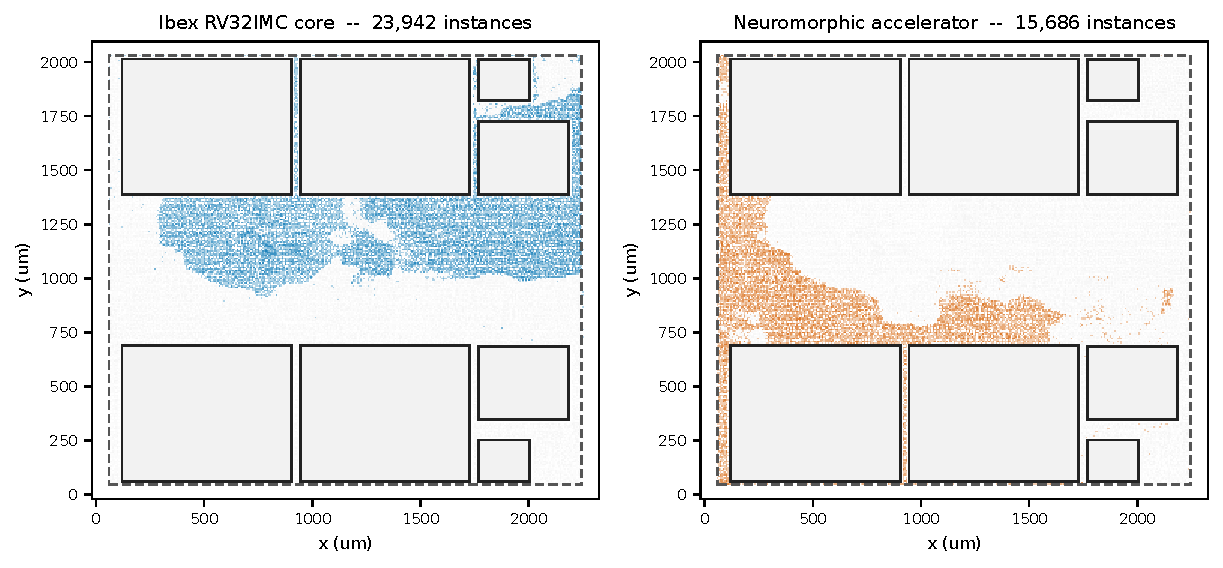
\includegraphics[width=\linewidth]{figures/layout_ibex_npu.pdf}
\caption{The two large blocks of the placed and routed
\code{soc\_top}: the Ibex core (left) and the neuromorphic accelerator
with the frozen die inside it (right), drawn against the same die
outline, core box and eight fixed vendor macros. Generated by
\code{thesis/figures/\allowbreak{}make\_layout\_figures.py} from a
sign-off run's placement database and netlist, which is the only
provenance that script records.}
\label{fig:npu-layout}
\end{figure}

\Cref{fig:npu-layout} answers ``where is the accelerator'' on a placed
and routed layout of the whole system-on-chip, and it must be read with
its method in mind. The die carries 168,592 instances --- the
attribution file the same script writes totals 168,584, a difference of
eight --- and after this flow's synthesis only 1,140 of those instance
names carry a dot at all, 632 of them the RAM's, with exactly one
passing the script's own top-level-block prefix test. A picture that
coloured only the named instances would colour one cell and answer the
question wrongly. Everything else is attributed by connectivity: nets
keep the hierarchical names Yosys did not create, so every net that
still carries a top-level prefix votes for that block; each anonymous
cell takes the block most of its pins' nets vote for; and two rounds of
neighbour propagation resolve the rest.

\textbf{The error bar is published with the picture and is 9.75\,\%.}
Of the 60,694 instances that are not fill, decap, tie or antenna cells,
5,916 could not be attributed and are drawn in grey rather than hidden;
107,890 fill, decap and diode instances are not drawn at all
(\code{thesis/figures/\allowbreak{}layout\_attribution.json}). The
accelerator's share is \textbf{15,686 instances} against the Ibex
core's 23,942 --- 25.8\,\% and 39.4\,\% of those 60,694.

The picture shows a block the placer spread rather than clustered: the
accelerator's cells occupy the lower half of the central channel
between the two macro rows, with the core taking the upper half, plus a
column running the full height of the die down its left edge. Apart
from the eight fixed macros, nothing here was told where to go.

It is also the physical statement of what the area measurements said.
At \dcite{51}{section 11}, on Yosys statistics against the
typical-corner library, the connection alone with the die black-boxed
was 2,723 cells and 57,805.4988 square micrometres and the whole
subsystem including the die was 12,421 cells and 209,739.0834 ---
\textbf{76.08\,\%} of the Ibex reference of 275,682.6198 by cell area.
Two hardening waves superseded those rows: the same recipe in
\dcite{56}{section 7} gives \textbf{3,416 cells and 67,338.0540} for
the connection and \textbf{13,148 cells, 2,092 flip-flops and
219,294.8478} for the whole subsystem. More than half of the connection
is its two event queues --- 53.5\,\% by area at the earlier measurement
--- expensive because they carry entry parity, pointer voting and drop
counting.

\section{What is open}

There is no second node and no router, so the mesh link is a frozen
interface with no implementation, and there are no descriptor rings
--- a ring would be a third bus master on a fabric whose fairness
property is written for two. Multi-pass sequencing is exercised by the
pilot's own suite and by nothing on the system-on-chip, where the tile
offset is written once, to zero. The weight path still enters the node
one register at a time, because that is the die's only weight port; the
flash controller changed where the words come from, not how they enter
(\dcite{51}{section 14}, corrected 2026-09-05).

Most of the connection's flip-flops are unprotected by decision --- the
transport's shift register, the engine's state, the window's captured
request and the frame guards --- and the queues' stored words carry
\code{aer\_fifo}'s detect-only entry parity and nothing beyond it. In
both cases the reason is a measurement rather than a budget. That queue
storage is 37.6\,\% of the connection's flip-flops now that the block
has grown, was 41.2\,\% when the campaign measured it, and is 53.5\,\%
of the area \dcite{51}{section 11} reports; it produced zero silent
wrong inferences in 100 draws, because occupancy is low and most of
those bits are storage nothing will read: a wave that started with the
biggest structure would have bought nothing. The largest site now left
is the engine's state register, at 7 of 20, which
\cref{eq:h5} has made load-bearing for a pin it was only implicitly
related to before.

One limit applies to everything measured here: every campaign in this
chapter is register-transfer, single-bit and flip-flop-only. No
back-annotated timing, no multi-bit strike, and no single-event
transient in combinational logic \cite{shivakumar2002} --- which matters because the strobe
gate \emph{is} combinational logic, so a transient on it is a failure
mode no instrument here can see. A gate-level netlist carrying the
connection has since been injected into --- \dcite{82}{} draws into the
accelerator's gated domain on a placed layout --- but at zero cell
delay and under a workload that never touches the accelerator
(\dcite{82}{section 8}).
